

\begin{figure}
    \centering
    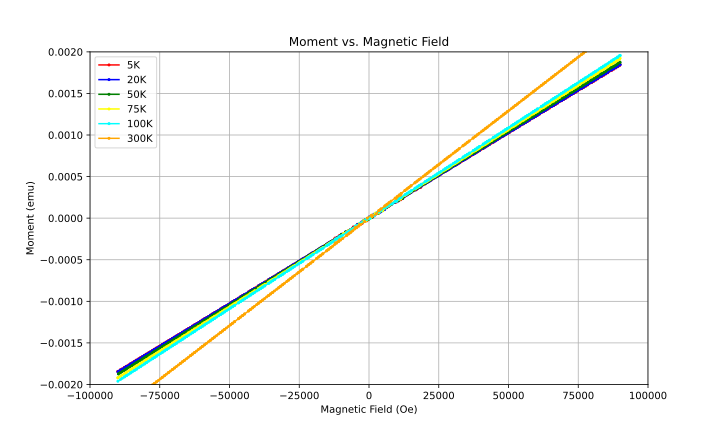
\includegraphics[width=\linewidth]{pdf_files/MvsH_all.pdf}
    \caption{M vs. H measurements for different temperatures along the b-axis. All R² values for linear fits of the data are 1.000 when using 4 significant figures, meaning the susceptibility is indeed linearly dependent on the applied field. The x-axis shows the magnetic field measured in Oe, while the y-axis shows the magnetic moment measured in emu.}
    \label{fig:MvsH-b}
\end{figure}
